\section{The California Report Card}
\subsection{System Description}
The California Report Card (CRC) is a web application that allows participants to advise the state government on timely policy issues.
When participants arrive at the application, they ``grade" the state on following six issues: (1) Implementation of the Affordable Care Act (``Obamacare"),
(2) Quality of K-12 public education, (3) Affordability of state colleges and universities, (4) Access to state services for undocumented immigrants, (5) Laws and regulations regarding recreational marijuana, and (6) Marriage rights for same-sex partners.
Grades are assigned on a thirteen point scale (A+,A,A-,...,D-,F).
These issues are posed in a fixed sequential order each with the same input scale.
Participants submit grades using a click-and-drag slider interface as illustrated in Figure \ref{grading-1}.
On mobile devices this slider requires the participants to touch and drag their finger to the desired grade.

\begin{figure}[h]
  \centering
    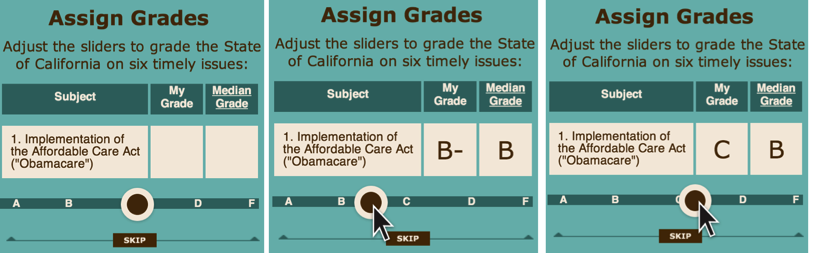
\includegraphics[width=\columnwidth]{../plots/grading-desc-1.png}
      \caption{Grading in the California Report Card. Participants enter grades on six timely issues facing the State of California. After entering their grades, the median grade over all participants is revealed. Participants have the option to change their grades after seeing the median.}
      \label{grading-1}
\end{figure}

Upon release of the slider, the CRC reveals the median grade for that issue over all prior participants.
Even after the median grade is revealed the slider is still active and participants can change their grades.
However, it is important to note that participants were not explicitly told that they could change their grades.
Another important observation is that participants who accessed the application at different times may have seen different median grades as they were calculated based on the data up to that point.
We recorded the initial grade, the median that the participant observed, and any subsequent changes along with timestamps for each of the events. 
Grading all of the six issues was not mandatory and participant had the option to skip any of the issues.

The CRC has an additional open-ended discussion phase where participant submit textual suggestions on future issues to include in the report card.
In this work, we focus on the first phase and defer an analysis of biases in the discussion phase to future work.

\subsection{Notation}
To analyze this data, we mapped these 13 grades onto a scale from 0 to 1, with 1 being an A+ and 0 being an F.
Let $P$ denote the set of all participants.
For each participant $p_j\in P$, we associate a 3-tuple of grades ($g_i[j]$, $m[j]$, $g_f[j]$) which represent the initial grade, median observed by the participant, and the final grade.
For each issue, we divided the participants into three subsets of $P$: ones who did not change their grades $P_n$, ones who changed $P_c$, and ones who skipped the question $P_s$.
Our primary objective is to test the distributional properties of rating tuples from participants in $P_n$ compared to those in $P_c$.

To ensure that all participants in the set $P_c$ had an opportunity to see the median grade and then react, we filtered this group using the timestamps. 
The median grade appears in the interface with an animation whose completion time varied between devices, so we set a grace period of 3 seconds before 
we categorized the participant into set $P_c$.  

For consistency, we use the same notation to describe participants in the reference survey. We denote the set of reference survey participants as set $R$, and each participant is associated with a 3-tuple ($g_i[j]$, $m[j]$, $g_f[j]$). However, since the reference survey does not reveal the aggregate statistics $g_i[j] = g_f[j]$  and $m[j]$ is the median of the prior participants (which is not shown).
